% -----------------------------------------------------------------------------
% Apêndices
% -----------------------------------------------------------------------------

\begin{apendicesenv}
    \partapendices

    % -------------------------------------------------------------------------
    % Primeiro apêndice
    % -------------------------------------------------------------------------

    \chapter{APÊNDICE DE INSTRUÇÃO}
    \label{apendice_a}

    É importante lembrar que a distinção entre apêndice e anexo está relacionada à autoria do material ou texto incluído.

    Se o conteúdo suplementar ou complementar for de sua própria autoria, ele deve ser classificado como apêndice. Por outro lado, se a autoria for de outra pessoa, o material deve ser apresentado como anexo.

    Se necessário, você pode incluir outros anexos em seu trabalho acadêmico. Para isso, basta copiar e colar este trecho no mesmo documento.

    Organize seus anexos de forma que cada um contenha apenas um tipo específico de conteúdo. Isso tornará a leitura e a compreensão mais fáceis para o leitor.

    % -------------------------------------------------------------------------
    % Novo apêndice
    % -------------------------------------------------------------------------

    \chapter{ILUSTRAÇÕES}
    \label{ilustracoes}

    A seguir, apresenta-se a maneira de incluir ilustrações no corpo do texto. De acordo com as normas, as figuras, tabelas, quadros, equações, algoritmos, diagramas, entre outros, são considerados tipos específicos de ilustrações.

    \section{TABELAS}
    \label{tabelas}

    Exemplo de tabela:

    \begin{table}[htb!]
\centering
\caption{Condições de contorno para velocidade e pressão.}
\label{tab:ccopenfoam}
\begin{tabular}{lcc}
\toprule

Condição         & Velocidade         & Pressão       \\ \midrule
Entrada          & fixedValue         & zeroGradient  \\
Saída            & zeroGradient       & fixedValue(0) \\
Paredes laterais & slip               & zeroGradient  \\
Rotor            & movingWallVelocity & zeroGradient  \\ \bottomrule
\end{tabular}
\fonte{Gabriel}
\end{table}

    \section{FIGURAS}

    A \autoref{fig_1} é automaticamente incluída na lista de figuras. Já a \autoref{fig_figura_exemplo2} apresenta um exemplo de figura que contém múltiplas imagens.

    \begin{figure}[!htb]
        \centering
        \caption{Domínio computacional empregado nas simulações.}
        \label{fig_1}
        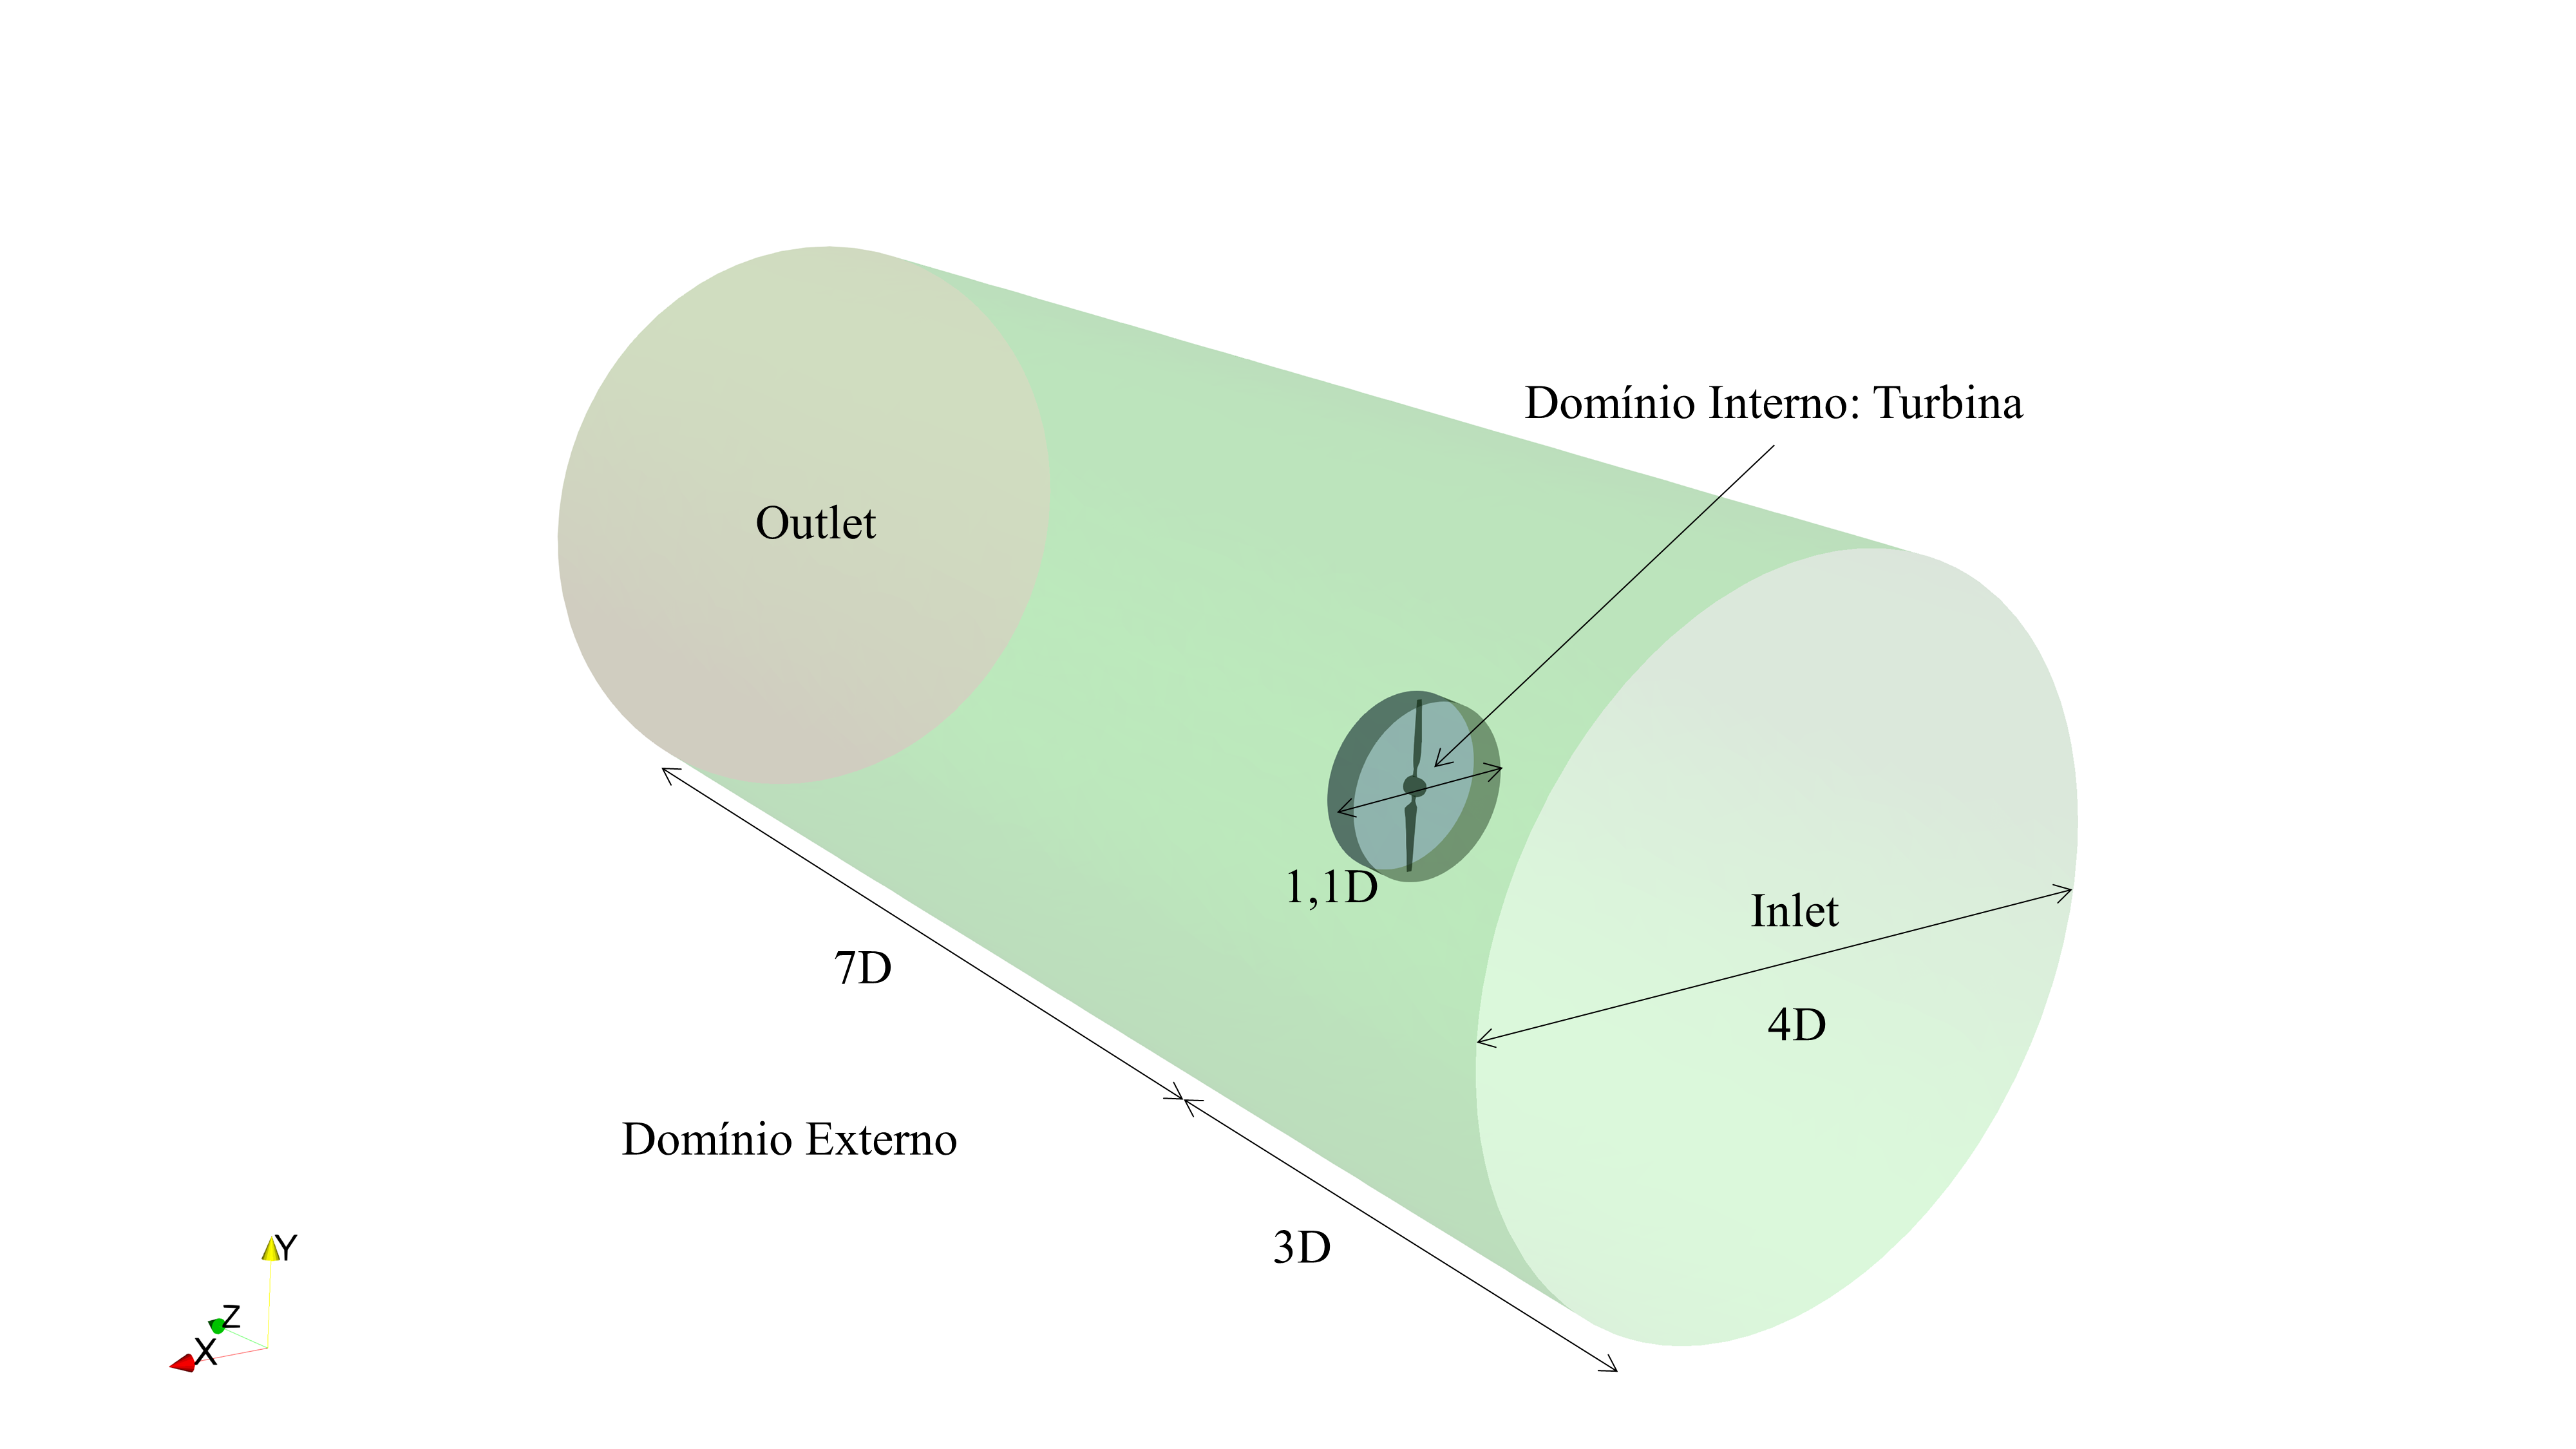
\includegraphics[width=0.75\textwidth]{figuras/domain.png}
        \fonte{Gabriel}
    \end{figure}

    \begin{figure}[!htb]
        \centering
        \caption{Exemplo.}
        \label{fig_figura_exemplo2}
        \subtop[][Exemplo.]{%
            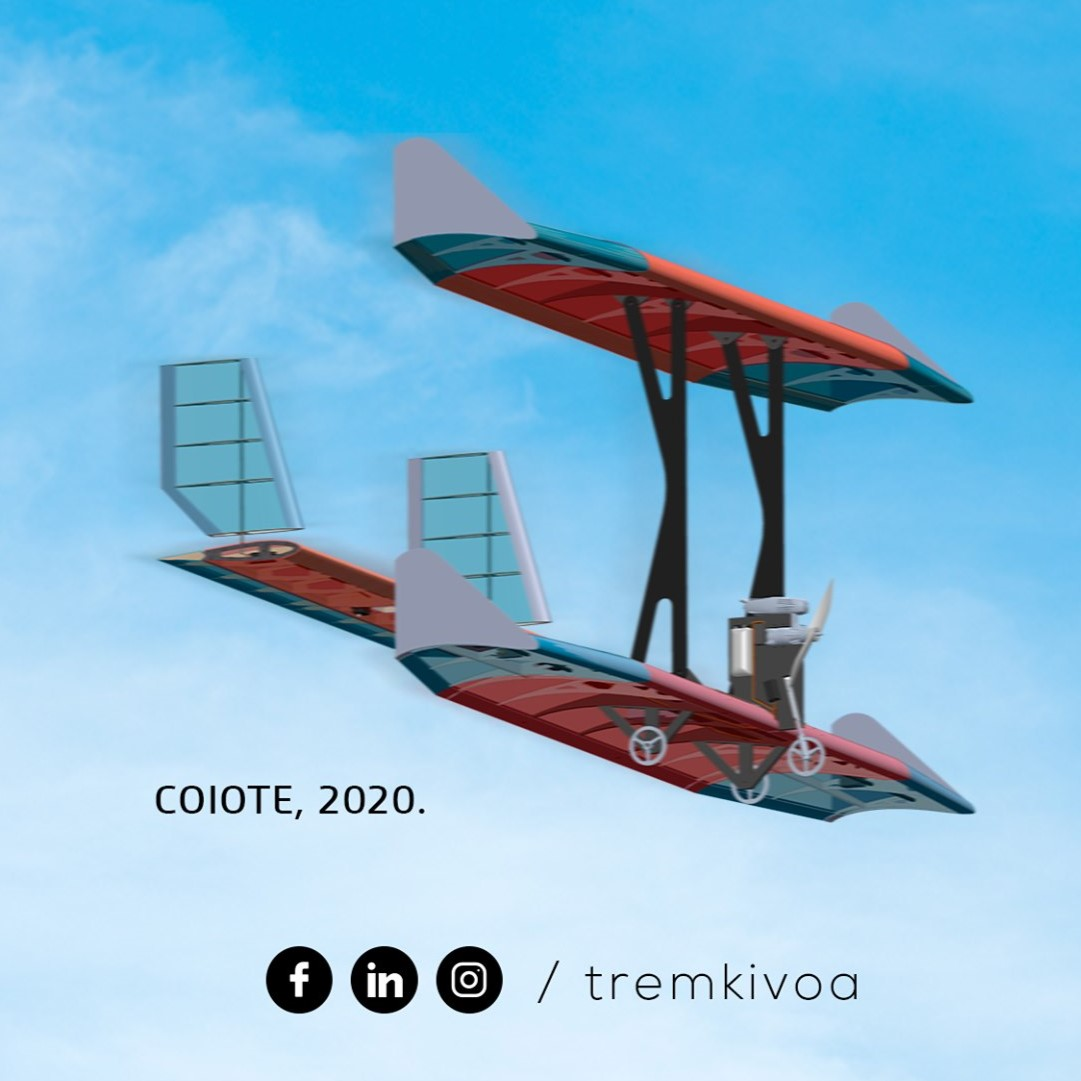
\includegraphics[scale=0.2]{figuras/tkv.jpg}%
        }\hspace{2ex}
        \subtop[][Exemplo.]{%
            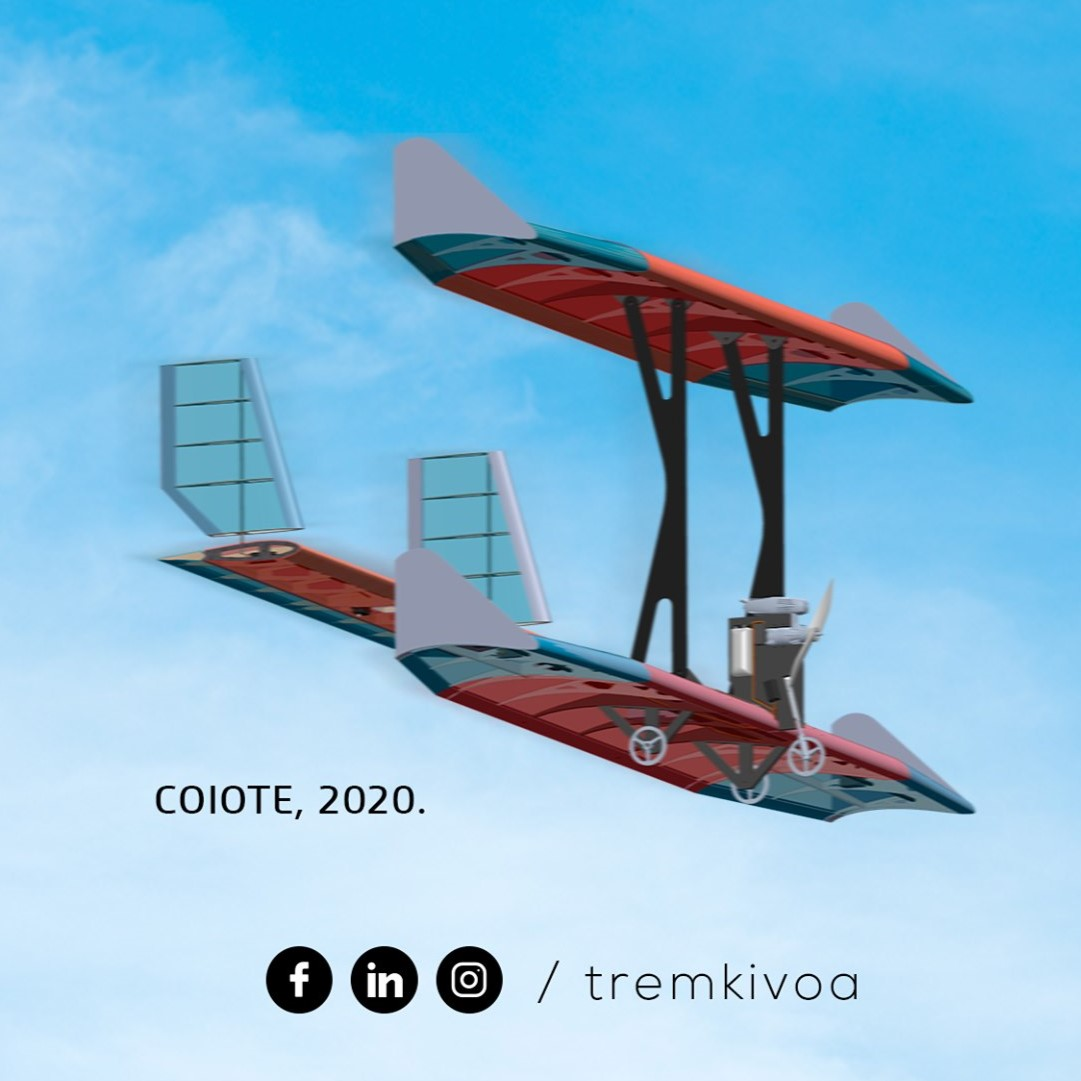
\includegraphics[scale=0.2]{figuras/tkv.jpg}%
        }\hspace{2ex}
        \subtop[][Exemplo.]{%
            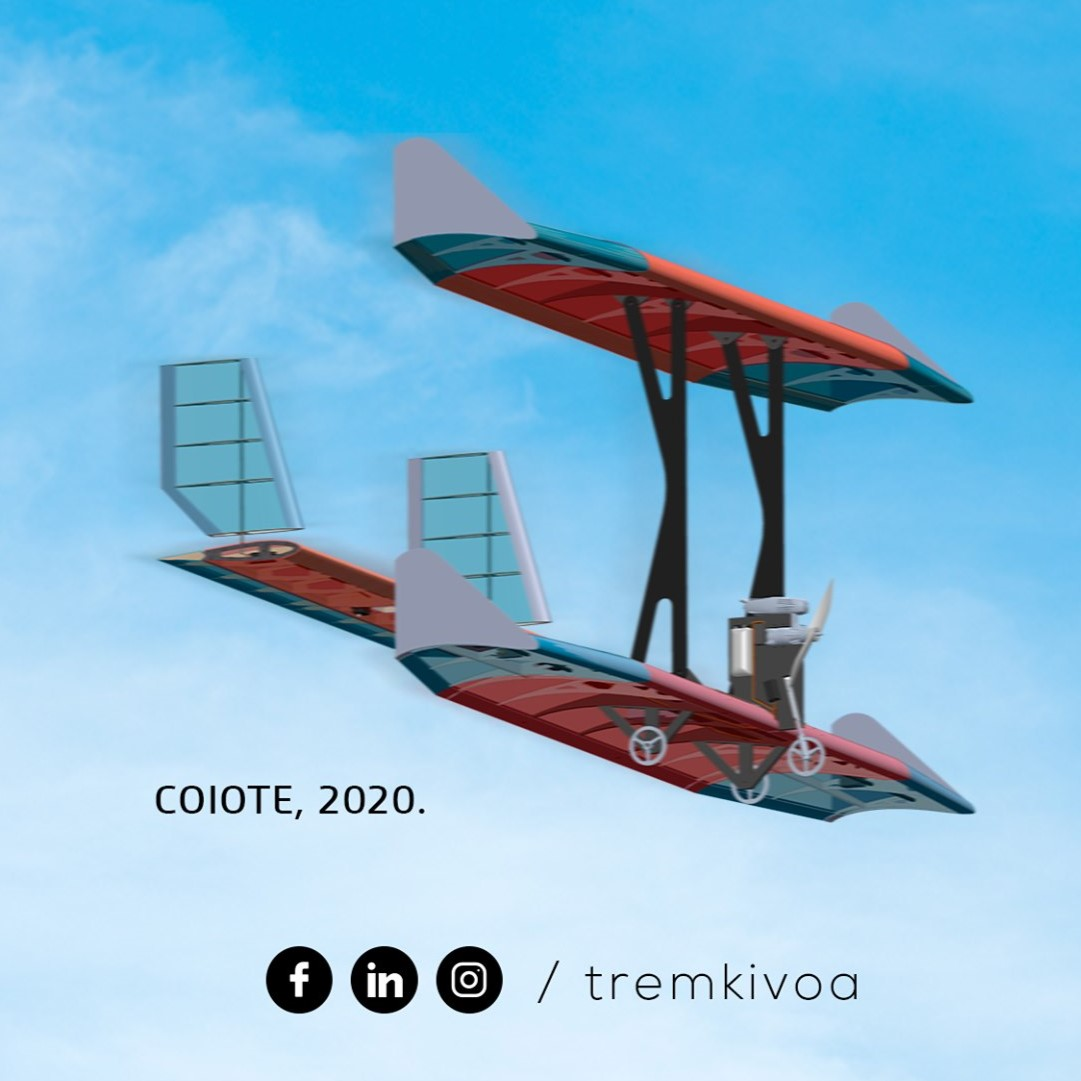
\includegraphics[scale=0.2]{figuras/tkv.jpg}%
        }
    \end{figure}

    \section{EQUAÇÕES}
    \label{equacoes}

   Para o modelo SST $k/\omega$, a energia turbulenta de fluxo livre e a taxa de dissipação da energia turbulenta foram calculadas pelas expressões:

    \begin{equation}
    k = \frac{3}{2} (U_\infty \cdot I)^{2}
    \label{eq41}
    \end{equation}
    e

    \begin{equation}
    \omega = \frac{k^{0.5}}{C_{\mu}^{0.25} L}, \\
    \epsilon =\frac{C_{\mu}^{0.75}k^{1.5}}{L},
    \label{eq42}
    \end{equation}
    onde $I$ = 5\% é a intensidade de turbulência e $L$ a escala de comprimento.

    \section{ALGORITMOS}
    \label{algoritmos}

    Os \index{algoritmos} algoritmos devem ser feitos segundo o \autoref{alg_verificacao_primo}:

    \begin{algorithm}
    \caption{Algoritmo para verificação de número primo (gerado pelo ChatGPT)}
    \label{alg_verificacao_primo}

    \KwIn{um número inteiro $n \geq 2$}
    \KwOut{verdadeiro se $n$ é primo, falso caso contrário}
    \If{$n = 2$}{ 
        \KwRet{verdadeiro} \\
    }
    \If{$n \mod 2 = 0$}{ 
        \KwRet{falso} \\
    }
    $i \leftarrow 3$ \\
    \While{$i \leq \sqrt{n}$}{
        \If{$n \mod i = 0$}{
            \KwRet{falso} \\
        }
        $i \leftarrow i + 2$ \\
    }
    \KwRet{verdadeiro} \\
    
    \end{algorithm}


\end{apendicesenv}
